\documentclass[a4paper, 12pt]{book}
\usepackage[english]{babel}
%\usepackage{mathpazo}
% page layout
\usepackage[left=20mm, right=20mm, top=25mm]{geometry}
\geometry{a4paper}

% appendices
\usepackage[toc,page]{appendix}

% images
\usepackage{graphicx}

% colored headings
\usepackage{xcolor}

% equation numbering
\usepackage{amsmath}
\makeatletter
\def\tagform@#1{\maketag@@@{\ignorespaces\sffamily(#1)\unskip\@@italiccorr}}
\makeatother

% bookmarks
\usepackage{bookmark}

% dedication
\newenvironment{dedication}
{\clearpage             % new page
 \thispagestyle{empty}  % no header and footer
 \vspace*{\stretch{1}}  % top space
 %\itshape               % italics text
 \raggedleft            % flush to the right margin
}
{\par                   % end paragraph
 \vspace{\stretch{3}}   % bottom space (3x top space)
 \clearpage             % finish page
}

% sectioning
\usepackage{titlesec}

% titleformat{name}
% {title style}
% {number style}
% {space between number and title}
% {before-title code}

\titleformat{\part}[display]
  {\normalfont \sffamily \bfseries \centering}
  {\color{red!70!black} \Large \partname \, \thepart}
  {10pt} % vertical spacing
  {\Huge}

\titleformat{\chapter}[display]
  {\normalfont \sffamily \bfseries}
  {\color{red!70!black} \large \chaptertitlename \, \thechapter}
  {1pt}
  {\titlerule[1pt] \vspace{7pt} \Huge}

\titleformat{\section}
  {\normalfont \sffamily \Large}
  {\color{blue!70!black} §\bfseries\thesection}
  {10pt}
  {\bfseries}

\titleformat{\subsection}
  {\normalfont \sffamily \large}
  {\color{blue!70!black} §\bfseries\thesubsection}
  {10pt}
  {\bfseries}

\titleformat{\subsubsection}
  {\normalfont \sffamily}
  {\color{red!70!black} §\bfseries\thesubsubsection}
  {10pt}
  {\bfseries}

\renewcommand{\appendixtocname}{\sffamily Appendices}
\renewcommand{\appendixpagename}{\sffamily \Huge \bfseries Appendices}

% custom table of contents
\usepackage{tocloft}

\renewcommand{\cfttoctitlefont}{\sffamily \Huge \bfseries} % title font
% part
\renewcommand{\cftpartfont}{\sffamily \large \bfseries}
\renewcommand{\cftpartpagefont}{\sffamily \large \bfseries}
\renewcommand{\cftpartpresnum}{\sffamily \color{red!70!black}}
% chapter
\renewcommand{\cftchapfont}{\sffamily \bfseries}
\renewcommand{\cftchappagefont}{\sffamily \bfseries}
\renewcommand{\cftchappresnum}{\sffamily \color{red!70!black}}
% section
\renewcommand{\cftsecfont}{\sffamily}
\renewcommand{\cftsecpagefont}{\sffamily}
\renewcommand{\cftsecpresnum}{\sffamily \color{blue!70!black}}
% subsection
\renewcommand{\cftsubsecfont}{\sffamily}
\renewcommand{\cftsubsecpagefont}{\sffamily}
\renewcommand{\cftsubsecpresnum}{\sffamily \color{blue!70!black}}

% unnumbered chapter
\titleformat{name = \chapter, numberless}[block]
  {\centering \sffamily \bfseries \Large}
  {}
  {0pt}
  {}

% headers and foooters
\usepackage{fancyhdr}
\setlength{\headheight}{15pt}

% part name
\let\Oldpart\part
\newcommand{\parttitle}{}
\renewcommand{\part}[1]{\Oldpart{#1}\renewcommand{\parttitle}{#1}}

% no random page numbers
\fancypagestyle{plain}{%
  \fancyhf{} % clear all header and footer fields
  \renewcommand{\headrulewidth}{0pt}
  \renewcommand{\footrulewidth}{0pt}
}

% custom headers and footers
\renewcommand{\chaptermark}[1]{\markboth{#1}{#1}}
\pagestyle{fancy}
\fancyhead{}
\fancyfoot{}

\fancypagestyle{body}{%
  \fancyhead[LE,RO]{\sffamily\thepage}%
  \fancyhead[LO]{\sffamily \color{blue!70!black}\chaptername\ \thechapter\color{black} :\ \leftmark}%
  \fancyhead[RE]{\sffamily \color{blue!70!black}\partname\ \thepart\color{black} :\ \parttitle}%
}

% special header for Introduction
\fancypagestyle{introd}{%
  \fancyhead[LE,RO]{\sffamily \thepage}%
  \fancyhead[RE,LO]{\sffamily \leftmark}%
}

% special header for Contents
\fancypagestyle{contents}{%
  \fancyhead[LE,RO]{\sffamily \thepage}%
  \fancyhead[RE,LO]{\sffamily }%
}

% special header for Appendix
\fancypagestyle{append}{%
  \fancyhead[LE,RO]{\sffamily \thepage}%
  \fancyhead[LO]{\sffamily \color{blue!70!black}\appendixname\ \thechapter \color{black}:\ \leftmark}%
  \fancyhead[RE]{\sffamily Appendices}%
}

% special header for Bibliography
\fancypagestyle{biblio}{%
  \fancyhead[LE,RO]{\sffamily \thepage}%
  \fancyhead[RE,LO]{\sffamily Bibliography}%
}

% no blank pages
\let\cleardoublepage\clearpage
% removes indentation
\setlength{\parindent}{0pt}
% add subsubsection numbering
\setcounter{secnumdepth}{3}

% math
\usepackage{amsmath}
\usepackage{amssymb}
\usepackage{amsfonts}
\usepackage{amsthm}
\usepackage{mathtools}
\usepackage{mathrsfs}
%\usepackage{tensor}

% physics
\usepackage{braket}

% chemistry
\usepackage{chemformula}

% footnotes
\usepackage{footnote}

% bold text

\newcommand{\bctxt}[1]{\textcolor{blue!70!black}{\textbf{#1}}}

\newcommand{\bcdef}[1]{\textcolor{green!35!black}{\textbf{#1}}}

\newcommand{\bcth}[1]{\textcolor{red!35!black}{\textbf{#1}}}

\newcommand{\bclemma}[1]{\textcolor{blue!35!black}{\textbf{#1}}}

\newcommand{\bcprop}[1]{\textcolor{cyan!35!black}{\textbf{#1}}}

\newcommand{\bcex}[1]{\textcolor{yellow!35!black}{\textbf{#1}}}

% fancy environments
\usepackage[many]{tcolorbox}
\BeforeBeginEnvironment{tcolorbox}{\savenotes}
\AfterEndEnvironment{tcolorbox}{\spewnotes}

\tcbuselibrary{theorems}

\NewTcbTheorem[number within=section]{definition}{Definition}{%
  enhanced,%
  breakable,%
  colback = green!5,%
  colframe = green!5,%
  coltitle = green!35!black,%
  fonttitle = \sffamily\bfseries,%
  sharp corners,%
  boxrule = 0pt,%
  detach title,%
  before upper = {\tcbtitle\\[4pt]},%
  left = 5pt,%
  right = 5pt,%
  top = 5pt,%
  bottom = 5pt,%
  separator sign none,%
  description delimiters parenthesis,%
  description font = \mdseries%
}{def}

\newtcbtheorem[number within=section]{theorem}{Theorem}{%
  enhanced,%
  breakable,%
  colback = red!5,%
  colframe = red!5,%
  coltitle = red!35!black,%
  fonttitle = \sffamily\bfseries,%
  sharp corners,%
  boxrule = 0pt,%
  detach title,%
  before upper = {\tcbtitle\\[4pt]},%
  left = 5pt,%
  right = 5pt,%
  top = 5pt,%
  bottom = 5pt,%
  separator sign none,%
  description delimiters parenthesis,%
  description font = \mdseries%
}{th}

\newtcbtheorem[number within=tcb@cnt@theorem]{corollary}{Corollary}{%
  enhanced,%
  breakable,%
  colback = red!5,%
  colframe = red!5,%
  coltitle = red!35!black,%
  fonttitle = \sffamily\bfseries,%
  sharp corners,%
  boxrule = 0pt,%
  detach title,%
  before upper = {\tcbtitle\\[4pt]},%
  left = 5pt,%
  right = 5pt,%
  top = 5pt,%
  bottom = 5pt,%
  separator sign none,%
  description delimiters parenthesis,%
  description font = \mdseries%
}{cor}

\newtcbtheorem[number within=section]{lemma}{Lemma}{%
  enhanced,%
  breakable,%
  colback = blue!5,%
  colframe = blue!5,%
  coltitle = blue!35!black,%
  fonttitle = \sffamily\bfseries,%
  sharp corners,%
  boxrule = 0pt,%
  detach title,%
  before upper = {\tcbtitle\\[4pt]},%
  left = 5pt,%
  right = 5pt,%
  top = 5pt,%
  bottom = 5pt,%
  separator sign none,%
  description delimiters parenthesis,%
  description font = \mdseries%
}{lemma}

\newtcbtheorem[number within=lemma]{lemcorollary}{Corollary}{%
  enhanced,%
  breakable,%
  colback = blue!5,%
  colframe = blue!5,%
  coltitle = blue!35!black,%
  fonttitle = \sffamily\bfseries,%
  sharp corners,%
  boxrule = 0pt,%
  detach title,%
  before upper = {\tcbtitle\\[4pt]},%
  left = 5pt,%
  right = 5pt,%
  top = 5pt,%
  bottom = 5pt,%
  separator sign none,%
  description delimiters parenthesis,%
  description font = \mdseries%
}{cor}

\newtcbtheorem[number within=section]{proposition}{Proposition}{%
  enhanced,%
  breakable,%
  colback = cyan!5,%
  colframe = cyan!5,%
  coltitle = cyan!35!black,%
  fonttitle = \sffamily\bfseries,%
  sharp corners,%
  boxrule = 0pt,%
  detach title,%
  before upper = {\tcbtitle\\[4pt]},%
  left = 5pt,%
  right = 5pt,%
  top = 5pt,%
  bottom = 5pt,%
  separator sign none,%
  description delimiters parenthesis,%
  description font = \mdseries%
}{prop}

\newtcbtheorem[number within=proposition]{propcorollary}{Corollary}{%
  enhanced,%
  breakable,%
  colback = cyan!5,%
  colframe = cyan!5,%
  coltitle = cyan!35!black,%
  fonttitle = \sffamily\bfseries,%
  sharp corners,%
  boxrule = 0pt,%
  detach title,%
  before upper = {\tcbtitle\\[4pt]},%
  left = 5pt,%
  right = 5pt,%
  top = 5pt,%
  bottom = 5pt,%
  separator sign none,%
  description delimiters parenthesis,%
  description font = \mdseries%
}{cor}

\newtcbtheorem[number within=section]{example}{Example}{%
  enhanced,%
  breakable,%
  colback = yellow!10,%
  colframe = yellow!5,%
  coltitle = yellow!35!black,%
  fonttitle = \sffamily\bfseries,%
  sharp corners,%
  boxrule = 0pt,%
  detach title,%
  before upper = {\tcbtitle\\[4pt]},%
  left = 5pt,%
  right = 5pt,%
  top = 5pt,%
  bottom = 5pt,%
  separator sign none,%
  description delimiters parenthesis,%
  description font = \mdseries%
}{ex}

\newtcolorbox{proofbox}{%
  enhanced,%
  breakable,%
  colback = black!5,%
  colframe = black!5,%
  sharp corners,%
  boxrule = 0pt,%
  left = 5pt,%
  right = 5pt,%
  top = 5pt,%
  bottom = 5pt,%
  borderline west = {1pt}{0pt}{black!70},%
}

% custom references
\newcommand{\eref}[1]{\textsf{Eq.\,\ref{#1}}}
\newcommand{\eeref}[2]{\textsf{Eq.\,\ref{#1}-\ref{#2}}}
\newcommand{\dref}[1]{\textsf{Def.\,\ref{#1}}}
\newcommand{\ddref}[2]{\textsf{Def.\,\ref{#1}-\ref{#2}}}
\newcommand{\tref}[1]{\textsf{Th.\,\ref{#1}}}
\newcommand{\pref}[1]{\textsf{Prop.\,\ref{#1}}}
\newcommand{\lref}[1]{\textsf{Lemma\,\ref{#1}}}
\newcommand{\exref}[1]{\textsf{Ex.\,\ref{#1}}}

\newcommand{\secref}[1]{\textcolor{red!70!black}{\textsf{§\ref{#1}}}}

% hyper-references
\usepackage{hyperref}
\hypersetup{
  colorlinks = true,
  urlcolor = cyan,
  % linkcolor defined directly in \toc environment
  citecolor = green!70!black,
}

\newcommand{\toc}{%
  \hypersetup{linkcolor = black}%
  \tableofcontents%
  \hypersetup{linkcolor = red!70!black}%
}

% extended integral symbols
\usepackage{esint}

% text
\newcommand{\virgolette}[1]{``\text{#1}"}
\newcommand{\tildetext}{\raise.17ex\hbox{$\scriptstyle\mathtt{\sim}$}}

% greek
\newcommand{\Chi}{\text{X}}

% custom math symbols
\newcommand{\abs}[1]{\left\lvert#1\right\rvert}
\newcommand{\norm}[1]{\left\lVert#1\right\rVert}
\newcommand{\sgn}[1]{\mathrm{sgn}\,#1}
\newcommand{\pa}{\partial}
\newcommand{\na}{\nabla}
\newcommand{\tens}[1]{\mathrm{#1}}
\newcommand{\defeq}{\mathrel{\vcenter{\baselineskip0.5ex \lineskiplimit0pt
                     \hbox{\scriptsize.}\hbox{\scriptsize.}}}%
                     =}
\newcommand{\eqdef}{=%
                     \mathrel{\vcenter{\baselineskip0.5ex \lineskiplimit0pt
                     \hbox{\scriptsize.}\hbox{\scriptsize.}}}}
\newcommand{\ve}[1]{\mathbf{#1}}
\newcommand{\hilb}{\mathscr{H}}
\newcommand{\fock}{\mathscr{F}}
\DeclareMathOperator{\diag}{diag}
\newcommand{\sqg}{\sqrt{\tens{g}}}
\newcommand{\sqgm}{\sqrt{-\tens{g}}}
\newcommand{\cm}{\mathcal{C}^{\infty}(\mathcal{M})}
\DeclareMathOperator{\lspan}{span}
\newcommand{\xm}{\mathfrak{X}(\mathcal{M})}
\DeclareMathOperator{\id}{id}
\newcommand{\ld}{\mathcal{L}}
\newcommand{\lm}[1]{\Lambda^{#1}(\mathcal{M})}
\newcommand{\hrm}[1]{\mathrm{Harm}^{#1}(\mathcal{M})}
\DeclareMathOperator{\ran}{ran}
\DeclareMathOperator{\tr}{tr}
\DeclareMathOperator{\Tr}{Tr}
\DeclareMathOperator{\End}{End}
\DeclareMathOperator{\im}{Im}
\newcommand{\dd}{\mathrm{d}}
\newcommand{\bs}[1]{\boldsymbol{#1}}
\newcommand{\dg}{^\dagger}
\DeclareMathOperator{\Aut}{Aut}
\DeclareMathOperator{\ad}{ad}
\DeclareMathOperator{\Ad}{Ad}
\newcommand{\lag}{\mathcal{L}}
\newcommand{\ham}{\mathcal{H}}
\newcommand{\act}{\mathcal{S}}
\newcommand{\normord}{\mathfrak{N}}
\newcommand{\tempord}{\mathfrak{T}}
\newcommand{\parity}{\mathcal{P}}
\newcommand{\chargec}{\mathcal{C}}
\newcommand{\timer}{\mathcal{T}}
\newcommand{\covder}{D}
\newcommand{\mat}{\mathcal{M}}
\newcommand{\smo}{\mathcal{O}}
\newcommand{\msb}{\overline{\text{MS}}}

\newcommand{\grad}{\boldsymbol{\nabla}}
\newcommand{\dive}{\boldsymbol{\nabla}\cdot}
\newcommand{\rot}{\boldsymbol{\nabla}\times}
\newcommand{\lap}{\triangle}

% small \overleftrightarrow
\makeatletter
\newcommand{\overleftrightsmallarrow}{\mathpalette{\overarrowsmall@\leftrightarrowfill@}}
\newcommand{\overrightsmallarrow}{\mathpalette{\overarrowsmall@\rightarrowfill@}}
\newcommand{\overleftsmallarrow}{\mathpalette{\overarrowsmall@\leftarrowfill@}}
\newcommand{\overarrowsmall@}[3]{%
  \vbox{%
    \ialign{%
      ##\crcr
      #1{\smaller@style{#2}}\crcr
      \noalign{\nointerlineskip}%
      $\m@th\hfil#2#3\hfil$\crcr
    }%
  }%
}
\def\smaller@style#1{%
  \ifx#1\displaystyle\scriptstyle\else
    \ifx#1\textstyle\scriptstyle\else
      \scriptscriptstyle
    \fi
  \fi
}
\makeatother
\newcommand{\smlra}[1]{\overleftrightsmallarrow{#1}}
\newcommand{\smla}[1]{\overleftsmallarrow{#1}}
\newcommand{\smra}[1]{\overrightsmallarrow{#1}}

% functions
\DeclareMathOperator{\sech}{sech}
\DeclareMathOperator{\Exp}{Exp}

% number sets
\newcommand{\N}{\mathbb{N}}
\newcommand{\Z}{\mathbb{Z}}
\newcommand{\Q}{\mathbb{Q}}
\newcommand{\R}{\mathbb{R}}
\newcommand{\C}{\mathbb{C}}
\newcommand{\K}{\mathbb{K}}

% groups
\newcommand{\Ot}{\mathrm{O}(3)}
\newcommand{\SOt}{\mathrm{SO}(3)}
\newcommand{\On}[1]{\mathrm{O}(#1)}
\newcommand{\SOn}[1]{\mathrm{SO}(#1)}
\newcommand{\Un}[1]{\mathrm{U}(#1)}
\newcommand{\SUn}[1]{\mathrm{SU}(#1)}
\newcommand{\GL}[1]{\mathrm{GL}(#1)}
\newcommand{\SL}[1]{\mathrm{SL}(#1)}

% units of measure
\newcommand{\m}{\,\mathrm{m}}
\newcommand{\ang}{\,\mathrm{\AA}}
\newcommand{\fm}{\,\mathrm{fm}}

\newcommand{\barn}{\,\mathrm{barn}}

\newcommand{\cels}{\,^{\circ}\mathrm{C}}

\newcommand{\ev}{\,\mathrm{eV}}
\newcommand{\kev}{\,\mathrm{keV}}
\newcommand{\mev}{\,\mathrm{MeV}}
\newcommand{\gev}{\,\mathrm{GeV}}
\newcommand{\tev}{\,\mathrm{TeV}}

% particles
\newcommand{\g}{\mathrm{g}}
\newcommand{\w}{\mathrm{W}}
\newcommand{\z}{\mathrm{Z}}

% custom title page
\newcommand{\customtitlepage}[7]{%
  \begin{titlepage}
    \centering
    % department logo at the top of the page
    
\includegraphics[width=0.75\textwidth]{imgs/unimi.jpg}\\
    \vspace{1cm} % ddjust the vertical space as needed
    {\large Bachelor's Degree in #1 \par} % degree title
    \vspace{1cm}
    %\hrule % horizontal line
    \vspace{1cm} % adjust the vertical space as needed
    {\large \sffamily \textbf{#2} \par} % thesis title (bold)
    \vspace{9cm} % adjust the vertical space as needed
    
    \begin{minipage}[H]{\textwidth}
      \small Supervisor: \\
      \normalsize #3 \\
      \vspace{1cm}
    \end{minipage}
    \begin{minipage}[t]{\textwidth}
      \raggedleft
      \small Student: \\
      \normalsize #4\\ % student name
      \normalsize Matr.: #5 % student number
    \end{minipage}

    % academic year section at the bottom of the page
    \vspace{\fill}
    {\normalsize Academic Year #6 \par}
    
  \end{titlepage}
}


\usepackage{overarrows}
\usepackage{slashed}
\usepackage{simpler-wick}

% \usepackage{tikz}
%\usepackage[compat=1.1.0]{tikz-feynman}


% bibliography

\usepackage{csquotes}
\usepackage[
backend = biber,
style = numeric-comp,
sorting = ynt
]{biblatex}
\addbibresource{bibl.bib}

\renewbibmacro{in:}{}

\AtEveryBibitem{%
	\clearfield{publisher}%
	\clearfield{month}%
	\clearfield{numpages}%
	\clearfield{issue}%
	\clearfield{isbn}%
}

\DeclareFieldFormat[book,article]{journaltitle}{#1}
\DeclareFieldFormat[book,article]{volume}{\mkbibbold{#1}}


\title{Thesis}
\author{Lucrezia Bioni}

\begin{document}

\frontmatter

\customtitlepage{Physics}{Next-to-Leading Order QCD Corrections to Scattering Processes Using $\theta$-Parameters in the Nested Soft-Collinear Subtraction Scheme}{Prof. Raoul Horst Röntsch}{Lucrezia Bioni}{13655A}{2024--2025}
\clearpage

\chapter*{Abstract}
\selectlanguage{english}
Perturbative Quantum Chromodynamics (QCD) corrections are essential for achieving high-precision theoretical predictions in particle physics, which makes them fundamental for interpreting data from modern particle accelerators, such as the Large Hadron Collider (LHC) at CERN. As experimental precision increases, theoretical predictions must also attain a level of accuracy that allows for meaningful comparisons with data. This requires extending perturbative calculations beyond the leading order (LO) to include next-to-leading order (NLO) and higher-order corrections in the strong coupling constant $\alpha_s$. These corrections account for crucial physical effects, such as real parton emissions and virtual loop contributions. \\
A significant challenge in calculating these higher-order corrections arises from the presence of infrared (IR) singularities, which occur when partons become soft or collinear. Although the sum of all contributions to a cross-section is finite, due to the cancellation of divergences between real emissions and virtual loops, each individual term is divergent. To manage these divergences and obtain finite, numerically stable results, it is necessary to introduce subtraction schemes that regularize the singularities locally in the phase space. \\
Over the past few decades, a variety of subtraction schemes have been developed for this purpose. Among them, the Nested Soft-Collinear (NSC) Subtraction Scheme has gained particular prominence due to its conceptual clarity, modular structure, and consistent extensibility from NLO to next-to-next-to-leading order (NNLO). The NSC scheme achieves a local cancellation of infrared singularities by factorizing soft and collinear limits in a nested manner. Furthermore, its modular nature allows the subtraction terms for complex processes to be built from a limited set of basic components, making it well-suited for implementation in automated Monte Carlo frameworks. \\
The aim of this thesis is to extend the NSC Subtraction Scheme by introducing a set of continuous parameters, called $\theta$-parameters, which systematically restrict the subtraction procedure to the singular, unresolved regions of phase space where soft and collinear singularities occur. Specifically, the parameter $\theta_s$ limits the energy of unresolved partons in the soft limit, while $\theta_i$ controls their angular separation in the collinear limit. The central motivation for this development is to improve numerical stability and efficiency in Monte Carlo integrations, particularly for multi-leg processes where redundant phase-space coverage can significantly slow down convergence. \\
The implementation and analytical study in this thesis demonstrate that introducing $\theta$-parameters preserves the theoretical consistency and modular nature of the NSC scheme. These parameters modify only the soft and collinear (real) contributions, while leaving the virtual corrections and those from PDF renormalization unchanged. Specifically, they appear in the $I_{\mathrm{S}}(\epsilon)$ and $I_{\mathrm{C}}(\epsilon)$ operators, which are part of the soft and collinear counterterms for the infrared-divergent scattering amplitudes. Crucially, the $\theta$-parameters do not compromise the cancellation of the infrared $1/\epsilon^2$ and $1/\epsilon$ poles when all contributions are summed. The coefficient of the $1/\epsilon^2$ pole in $I_{\mathrm{S}}(\epsilon)$ is independent of any parameter, and, while the coefficients of the $1/\epsilon$ poles in $I_{\mathrm{S}}(\epsilon)$ and $I_{\mathrm{C}}(\epsilon)$ depend on $\theta_s$, this dependence cancels out in their sum. This confirms that the modified NSC scheme yields the same physical cross-sections as the standard one. \\
Therefore, the study presented in this thesis contributes to the ongoing effort to improve the efficiency and reliability of higher-order QCD computations. Such improvements are fundamental to continue testing the Standard Model and searching for new Physics beyond its confines.


\newpage

\toc

\pagestyle{contents}

\mainmatter

\chapter{Introduction}

\section{The Standard Model}

As Aristotle stated, women and men began to philosophize due to wonder. From antiquity, a profound sense of astonishment towards the natural world has driven humans to investigate phenomenological reality. This drive is so profound and innate in humanity that – starting with the first philosophers, called ``Pre-Socratics"  or ``natural philosophers" – it led them to inquire into the nature of the ``archè" ($\acute{\alpha}\rho\chi\acute{\eta}$), the primordial principle and fundamental constituent underlying all of nature. This enduring pursuit of fundamental knowledge evolved through the centuries and, in the last one, culminated in the experimental discovery of a multitude of subatomic particles, now understood to be the elementary constituents of matter. Their proliferation was such that it prompted the noted physicist Enrico Fermi to remark: ``If I could remember the names of all these particles, I'd be a botanist". This apparent complexity, however, has been successfully resolved through the development of a robust theoretical framework that classifies these particles and describes their interactions via gauge theories: the Standard Model (SM). \\
The SM is formulated within the mathematical framework of Quantum Field Theory (QFT), which unifies the principles of Quantum Mechanics and Special Relativity to describe phenomena at high energies and subatomic scales. Its predictions have been rigorously tested and confirmed by experiments, most notably with the discovery of the Higgs boson in 2012.  Despite its success, there are significant efforts to discover Physics beyond the SM. This is driven not only by the natural attempt at falsification that should be applied to every scientific theory, but also by several phenomena that the model cannot explain. These include the existence of dark matter and dark energy, the observed matter-antimatter asymmetry, and the origin of neutrino masses \cite{Campbell:2017}. \\
\subsection{Collider physics}
The principal method of research in high-energy physics is collider physics \cite{ellis}. Using colliders, it is possible to artificially accelerate particles and reach the highest available center-of-mass energy. Operating at the energy frontier is crucial: higher-energy collisions enable events with greater momentum transfer and energy deposition. These events are essential because concentrating significant energy within a tiny volume allows us to excite new, heavy elementary particles from the vacuum, and study their properties. Experiments at the energy frontier are conducted at the Large Hadron Collider (LHC) at CERN: in a 27-kilometer ring, proton beams collide at a center-of-mass energy of 13 TeV. Although these energy scales have allowed us to study the known fundamental interactions – with the exception of gravity – in great detail, they have not been sufficient for the discovery of new particles. Since increasing the energy of the colliding particles is not feasible with existing technology, the focus of collider experiments in the next decade will shift towards higher experimental precision. However, testing the Standard Model with experimental results necessitates reliable theoretical predictions for hadron collider processes. \\
\section{QCD and hard scattering processes}
A theoretical description of hadron collisions is complicated primarily by our limited knowledge of the strong force, which binds the elementary constituents of hadrons. A way to overcome this obstacle becomes manifest when we consider how hadrons collide at high energies \cite{Asteriadis2020}. Typically, they undergo either elastic scattering or diffractive dissociation: in the first case, they collide but remain intact; in the second, they disintegrate into a small number of hadrons. However, on rare occasions, a more interesting phenomenon can occur: the elementary partons that compose the hadrons can interact and exchange a large amount of momentum. This is the case in so-called ``hard scattering processes", and their importance is related to a significant feature of the strong force: asymptotic freedom. The essence of this property is the weakening of the colour force at short distances \cite{ellis}, which is precisely what allows for a perturbative description of the strong interaction and the use well-defined approximation methods. Therefore, in these cases, it is possible to organize the calculation into different orders: 
\begin{itemize}
    \item the Leading Order (LO), which describes the simplest, tree-level interaction;
    \item the Next-to-Leading Order (NLO), which adds important quantum corrections from virtual particle loops and the emission of an additional parton (real radiation);
    \item the Next-to-Next-to-Leading Order (NNLO), which includes two-loop, one-loop with real emission, and double real-emission diagrams; and so on.
\end{itemize}

\subsection{Hadronic cross-section and factorization theorem}
Strong interactions are described by Quantum Chromodynamics (QCD), a non-abelian gauge theory based on the SU(3) symmetry group. Their strength is given by the coupling constant, which is on the order of $\alpha_{\text{S}}\sim0.1$\footnote{This value is energy-dependent; $\alpha_{\text{S}}\sim0.1$ is typical at energies around 100 GeV.}: therefore, the strong force is about ten times stronger than the electromagnetic one (whose coupling constant is $\alpha\sim1/137$). The QCD Lagrangian is not analytically solvable, making it extremely difficult to understand proton dynamics from first principles. Therefore, an approach that focuses on the elementary quark and gluon fields, which are the fundamental degrees of freedom in QCD, is highly valuable. However, due to quark confinement\footnote{Quark confinement is the phenomenon that prevents quarks and gluons from propagating as free particles over macroscopic distances.}, this approach is only sensible at short distances. In this high-energy regime, the interacting partons can be approximated as being nearly free. \\
A framework for describing these short-distance hard scattering processes is provided by the collinear factorization theorem \cite{Collins:1987pm}. Within this framework, colliding hadrons are treated as beams of partons, each carrying a certain fraction of the hadron's total momentum. The probability of finding a parton with a specific energy fraction is encoded in the Parton Distribution Functions (PDFs). These functions are universal, meaning they are independent of the specific scattering process being studied. Consequently, PDFs can be measured in one set of experiments and then used to make predictions for many others \cite{Melnikov2018}. The short-distance interaction of partons produces final states composed of Standard Model particles, such as leptons, gauge bosons, and additional QCD partons. The final-state partons, which are the direct products of the perturbative calculation, cannot be observed directly due to confinement. Instead, they evolve into collimated sprays of hadrons \cite{Salam:2010nqg}. We interpret these partons as the seeds of hadronic jets and define the resulting sprays as jets themselves. At high energies, the properties of these jets are largely determined by the perturbative dynamics of their initiating parton and are only mildly affected by non-perturbative QCD effects. \\
The production cross section for final states involving QCD jets and other Standard Model particles in hard hadronic collisions is thus given by
\begin{equation}
    \text{d}\sigma = \sum_{a, b} \int_0^1 \text{d}x_1 \text{d}x_2 \, f_{a}(x_1, \mu_\text{F}) \, f_{b}(x_2,\mu_\text{F}) \, \text{d}\hat \sigma_{a,b}(x_1,x_2,\mu_\text{F},\mu_\text{R};\mathcal{O}) \, \left(1+ \mathcal{O}\left(\frac{\Lambda_{\text{QCD}}}{Q} \right)^n \right), \qquad n\geq1
    \label{fact-theor}
\end{equation}
where $f_{a,b}$ are the parton distribution functions mentioned above, and $\mathcal{O}$ is an infrared-finite observable. \\
The asymptotic freedom of QCD is what enables a perturbative description of the strong interaction. However, it is crucial to recognize that the precise mechanism allowing us to decouple the motion of partons from the proton's dynamics is the separation of energy scales involved. Interactions in the Standard Model typically probe energy scales on the order of $Q \sim 100  \, \text{GeV} - 1 \, \text{TeV}$, while the characteristic energy scale of hadronic structure and confinement is significantly lower, $\Lambda_{\text{QCD}} \sim 100 \, \text{MeV}$. This results in a small ratio, $\Lambda_{\text{QCD}}/Q \sim 10^{-2}$. The exact power $n$ with which non-perturbative effects are suppressed is not always immediately evident. In many practical applications, the leading power is $n=2$, implying that the theoretical error committed by factorizing the non-perturbative physics is of order $\mathcal{O}(\alpha_{\text{S}}^4) \sim 10^{-3}$ for $\alpha_S \sim 0.1$. \\
This formalism establishes a clear distinction between the short-distance perturbative process and the long-distance non-perturbative physics. The boundary between these two regimes is defined by the factorization scale ($\mu_\text{F}$). Processes with a momentum transfer $Q > \mu_\text{F}$ are treated as the hard scatter of point-like partons, calculable within perturbation theory. Physics at scales $Q < \mu_\text{F}$, which describes how the partons are bound within the proton, is incorporated into the non-perturbative Parton Distribution Functions (PDFs). \\
The other scale present in the factorized cross-section in Eq. \ref{fact-theor} is the renormalization scale ($\mu_\text{R}$). Its necessity arises because the calculation of partonic interactions in QCD using Feynman diagrams often results in ultraviolet (UV) divergences. These infinities do not indicate a fundamental error in the theory, but suggest a distinction between the bare parameters in the Lagrangian and physically observable quantities. The process of renormalization allows us to absorb these divergences into a redefinition of the Lagrangian's parameters, providing finite expressions for measurable quantities. The consequence of this procedure is that the coupling constant becomes a function of the energy scale, a phenomenon known as ``running" \cite{ellis}. The renormalization scale $\mu_\text{R}$ is the energy at which the coupling constant is defined, thereby encapsulating the quantum corrections of the theory. \\
For simple processes dominated by a single characteristic energy scale $\mu$, it is conventional to set both $\mu_\text{F}$ and $\mu_\text{R}$ equal to that scale \cite{Campbell:2017}. Therefore, throughout this thesis, we set $\mu_\text{F} = \mu_\text{R} = \mu$. Since their exact values are arbitrary, a physical prediction (like a cross-section) must be independent of them\footnote{However, cross-sections calculated within fixed-order perturbative expansions exhibit a dependence on both the renormalization and factorization scales, $\mu$}.  \\
Referring to Eq. \ref{fact-theor}, we can state that only the left-hand side represents a physically measurable quantity. The right-hand side, in contrast, consists of unobservable components: the parton distribution functions (PDFs), which are extracted from experimental data, and the partonic cross-section $\mathrm{d}\hat{\sigma}_{a,b}$, which is calculable within perturbation theory. It is therefore essential to understand how this latter quantity is computed.

\begin{figure}[!ht]
	\centering
	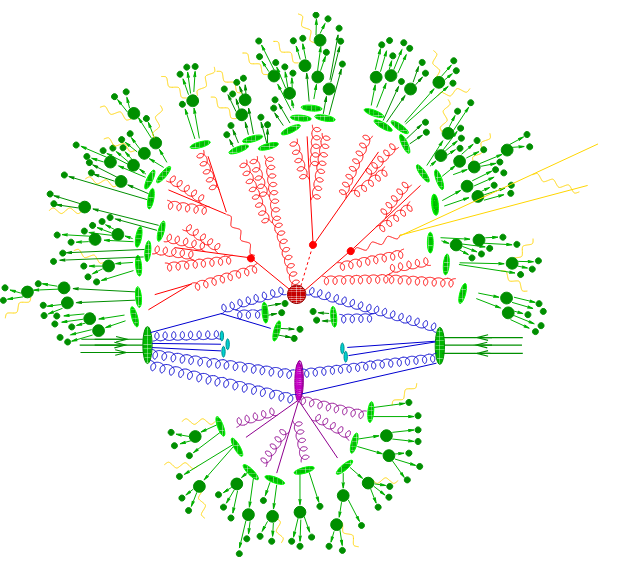
\includegraphics[width=0.7\textwidth]{imgs/hadron-collision.png}
	\caption{Sktetch of an hard hadron-hadron collision at a collider like the LHC. The central red blob represents the hard interaction, a high-energy collision between two partons, calculable using perturbative QCD. The incoming and outgoing partons emit initial-state (blue) and final-state (red) radiation, producing many secondary particles. Softer underlying event activity (purple) arises from additional partonic interactions within the protons. A key feature is the hierarchy of energy scales: the hard process occurs at high energies ($Q>\Lambda_{\text{QCD}}$), while subsequent radiation and hadronization (green) take place at progressively lower scales, eventually transitioning to non-perturbative physics around $\Lambda_{\text{QCD}}$. Figure from \cite{Hoeche:2014}.}
	\label{hadron-collision}
\end{figure}

\subsection{Partonic cross-section}
We consider the inclusive\footnote{The inclusive cross-section counts every collision event that creates a specific particle, whether it appears alone, with jets, or with any other additional radiation. It gives the total production rate, ignoring the details of what else is produced alongside it.} production of $N$ jets at a hadron collider, together with a color-neutral system $X$
\begin{equation}
    pp \rightarrow X + N \, \mathrm{jets}  \, .
\end{equation}
The partonic cros section $\mathrm{d}\hat{\sigma}_{a,b}$ in Eq. \ref{fact-theor} can be expanded in powers of the strong and the electroweak coupling constants, $\alpha_{\text{S}}$ and $\alpha$,
\begin{equation}
    \text{d} \hat{\sigma}_{a,b} = \text{d} \hat{\sigma}_{a,b}^{(0,0)} + \alpha_s \text{d} \hat{\sigma}_{a,b}^{(1,0)} + \alpha_s^2 \text{d} \hat{\sigma}_{a,b}^{(2,0)} + \alpha_s^3 \text{d} \hat{\sigma}_{a,b}^{(3,0)} + \alpha \text{d} \hat{\sigma}_{a,b}^{(0,1)} + \alpha \alpha_s \text{d} \hat{\sigma}_{a,b}^{(1,1)} + \dots .
\end{equation}
Due to the different values of the coupling constants, at the same order they have a different impact on the final result: at NLO, QCD corrections account for $10\%$, while EW account for $1\%$; at NNLO, QCD corrections account for $1\%$. Throughout this thesis, we will focus on the calculation of NLO QCD corrections. \\
The first term in this expansion $\text{d} \hat{\sigma}_{a,b}^{(0,0)} \equiv \text{d} \hat{\sigma}_{a,b}^{\text{LO}}$ is called Leading Order (LO), and it is defined as \cite{Devoto:2025jql}
\begin{equation}
    2s_{a,b} \, \text{d} \hat{\sigma}_{a,b}^{\text{LO}} = \langle F^{ab}_{\mathrm{LM}}[\dots] \rangle = \mathcal{N} \int \mathrm{d}\Phi (2\pi)^4 \delta^{(4)}(p_\mathcal{H_f}+p_X-p_a-p_b) \left|\mathcal{M}_0(p_a,p_b;p_{\mathcal{H}_f},p_X) \right|^2 \mathcal{O}(p_\mathcal{H},p_X).
    \label{leading-order}
\end{equation}
With $\mathcal{H}_f$, we denote the list of final-state resolved particles, and $p_{\mathcal{H}_f}$ is their momentum, while $p_X$ denotes the momentum of the color-singlet in the hard process. $\mathcal{N}$ is a normalization factor: it takes into account color and spin averages as well as symmetry factors. With $s_{a,b}$, we express the partonic center-of-mass energy squared: $s=(p_a+p_b)^2=2 p_a\cdot p_b$, considering massless partons. $\mathcal{M}_0$ is the matrix element for the process considered, $\mathcal{O}$ is an IR-safe observable which ensures that the final state contains at least $N$ resolved jets, and $\mathrm{d}\Phi$ is the Lorentz-invariant phase space for the final-state particles
\begin{equation}
    \mathrm{d}\Phi=\prod_{i=3}^{N_p} [\mathrm{d}p_i], \qquad [\mathrm{d}p_i]=\frac{\mathrm{d}^3p_i}{(2\pi)^32E_i},
\end{equation}
where $N_p=N+2$ is the number of initial- and final-state partons, and $[\mathrm{d}p_i]$ is the phase-space element of a final-state parton $i$. Moreover, in Eq. \ref{leading-order}, summation over spins and colors of final-state partons, and averaging over spins and colors of initial-state partons are assumed.  \\
The function $F^{ab}_{\mathrm{LM}}$ that appears in Eq. \ref{leading-order} is defined as in Section 2 of \cite{Devoto:2023rpv}
\begin{equation}
    F^{ab}_{\mathrm{LM}} = \mathrm{dLips}_X |\mathcal{M}_0|^2 \, \mathcal{O}
    \label{flm}
\end{equation}
where $\mathrm{dLips}_X$ is the Lorentz-invariant phase space for the colorless particle $X$, including the momentum-conserving delta function. The integration over the final-state phase space of Eq. \ref{flm}, denoted with the angular brackets $\langle\dots\rangle$, gives exactly Eq. \ref{leading-order}. \\
At leading order (LO), calculations are performed directly. The tree-level matrix elements can be computed easily using helicity techniques and colour-subamplitude decompositions \cite{Altarelli:1977zs}, and are then integrated, either numerically or analytically. \\



QCD corrections, infrared poles and their cancellation. L'aggiunta di correzioni è ciò che consente di tenere conto di effetti a lunga distanza, e far sì che i risultati forniti non siano validi solo a distanze brevi.\\
Le divergenze costituiscono termini non perturbativi nel nostro conto perturbativo, pertanto è importante trovare un modo di trattarle.
\\


Fixed order corrections \\
There are two types of corrections: virtual and real. \\
There are two challenges in computing corrections beyond LO: computing (multi)-loop virtual amplitudes and treating infrared divergences. 
\\
Nowadays, also next-to-leading order (NLO) calculations are feasible in a direct man-
ner, as witnessed by the accelerated production rate of new NLO computations [3]. This
achievement is the result of much theoretical progress in the last few years. This progress
regards both efficient techniques for the evaluation of one-loop matrix elements [4] and com-
pletely general algorithms [5–8] to handle and cancel infrared singularities when combining
tree-level and one-loop contributions in the evaluation of physical quantities. \\
 (Melnikov's notes ) \cite{Melnikov2018} \\
Asymptotic freedom is central to our ability to describe hard scattering processes at the LHC in
QCD perturbative theory since the smallness of the coupling constant is a pre-requisite for the success of
perturbative description. Note that for typical LHC processes the strong coupling constant is small but not
tiny. This implies that quite often QCD corrections need to be computed to higher orders to claim high
precision. The technology for computing next-to-leading QCD corrections to many processes of interest
was developed in mid 1990s [10,11] and an important ingredient was added about ten years ago [12,13].
Since then, the development of theoretical methods for next-to-next-to-leading order (NNLO) computa-
tions became of great interest to the community of theorists interested in precision LHC phenomenology.
Very recently, we have seen the emergence of several key technologies for NNLO computations [14] and
dramatic increase in the number of their applications to LHC physics [15].
The use of QCD to describe hard scattering processes at the LHC is intimately connected with
the detailed understanding of how scattering amplitudes behave in the so-called soft and collinear limits.
The soft limit corresponds to a situation where energy of an emitted gluon becomes small



\clearpage

\chapter{NLO QCD corrections in the NSC Subtraction Scheme}

\section{Draft}

\clearpage

\chapter{NLO QCD corrections with $\theta$-parameters in the NSC Subtraction Scheme}

\section{Draft}

\clearpage

\bookmarksetupnext{level = -1}
\begin{appendices}
\pagestyle{append}

\chapter{Draft appendix}

\section{Draft}

Lorem ipsum dolor sit amet \cite{pauli}.

\clearpage
\end{appendices}

\bookmarksetupnext{level = -1}
\pagestyle{biblio}
\printbibliography[heading = bibintoc, title = {Bibliography}]

\end{document}